\documentclass{beamer}

% Top-aligning columns within a top-aligned frame
% https://tex.stackexchange.com/questions/16447/beamer-top-aligning-columns-within-a-top-aligned-frame
\makeatletter
\newenvironment{myitemize}{%
   \setlength{\topsep}{0pt}
   \setlength{\partopsep}{0pt}
   \renewcommand*{\@listi}{\leftmargin\leftmargini \parsep\z@ \topsep\z@ \itemsep\z@}
   \let\@listI\@listi
   \itemize
}{\enditemize}
\makeatother  

\usepackage[USenglish]{babel}
\usepackage[utf8]{inputenc}
\usepackage{amssymb, amsmath}
\usepackage{bm}
\usepackage{color}
\usepackage{tikz}
\usepackage{url}

\definecolor{links}{HTML}{2A1B81}
\hypersetup{colorlinks,linkcolor=,urlcolor=links}

\usetheme{Boadilla}

\bibliographystyle{apalike}
% make bibliography entries smaller
%\renewcommand\bibfont{\scriptsize}
% Now get rid of all the colours
\setbeamercolor*{bibliography entry title}{fg=black}
\setbeamercolor*{bibliography entry author}{fg=black}
\setbeamercolor*{bibliography entry location}{fg=black}
\setbeamercolor*{bibliography entry note}{fg=black}

\newcommand{\lnorm}[1]{\left\lVert#1\right\rVert^2}
\newcommand{\norm}[1]{\left\lVert#1\right\rVert}

% and kill the abominable icon
\setbeamertemplate{bibliography item}{}

\begin{document}
\title[VQ-VAE]{Neural Discrete Representation Learning}  
\author{Radek Bartyzal}
\date{2. 2. 2021} 
\institute{GLAMI AI}

\frame{\titlepage} 

%--------- END Frame 12 -------------
\begin{frame}{Motivation}

Paper is by Google DeepMind from 2018.
\vfill

\textbf{Goal}:
Learn useful representations without supervision.
\vfill
\textbf{Contribution}:
Generative model that learns \textbf{discrete} representations.
\vfill
\textbf{Why discrete?}
Discrete representations are a natural fit for complex reasoning, planning and predictive learning.

\end{frame}
%--------- END Frame 12 -------------
\begin{frame}{Variational AutoEncoders = VAE}

\begin{figure}[h]
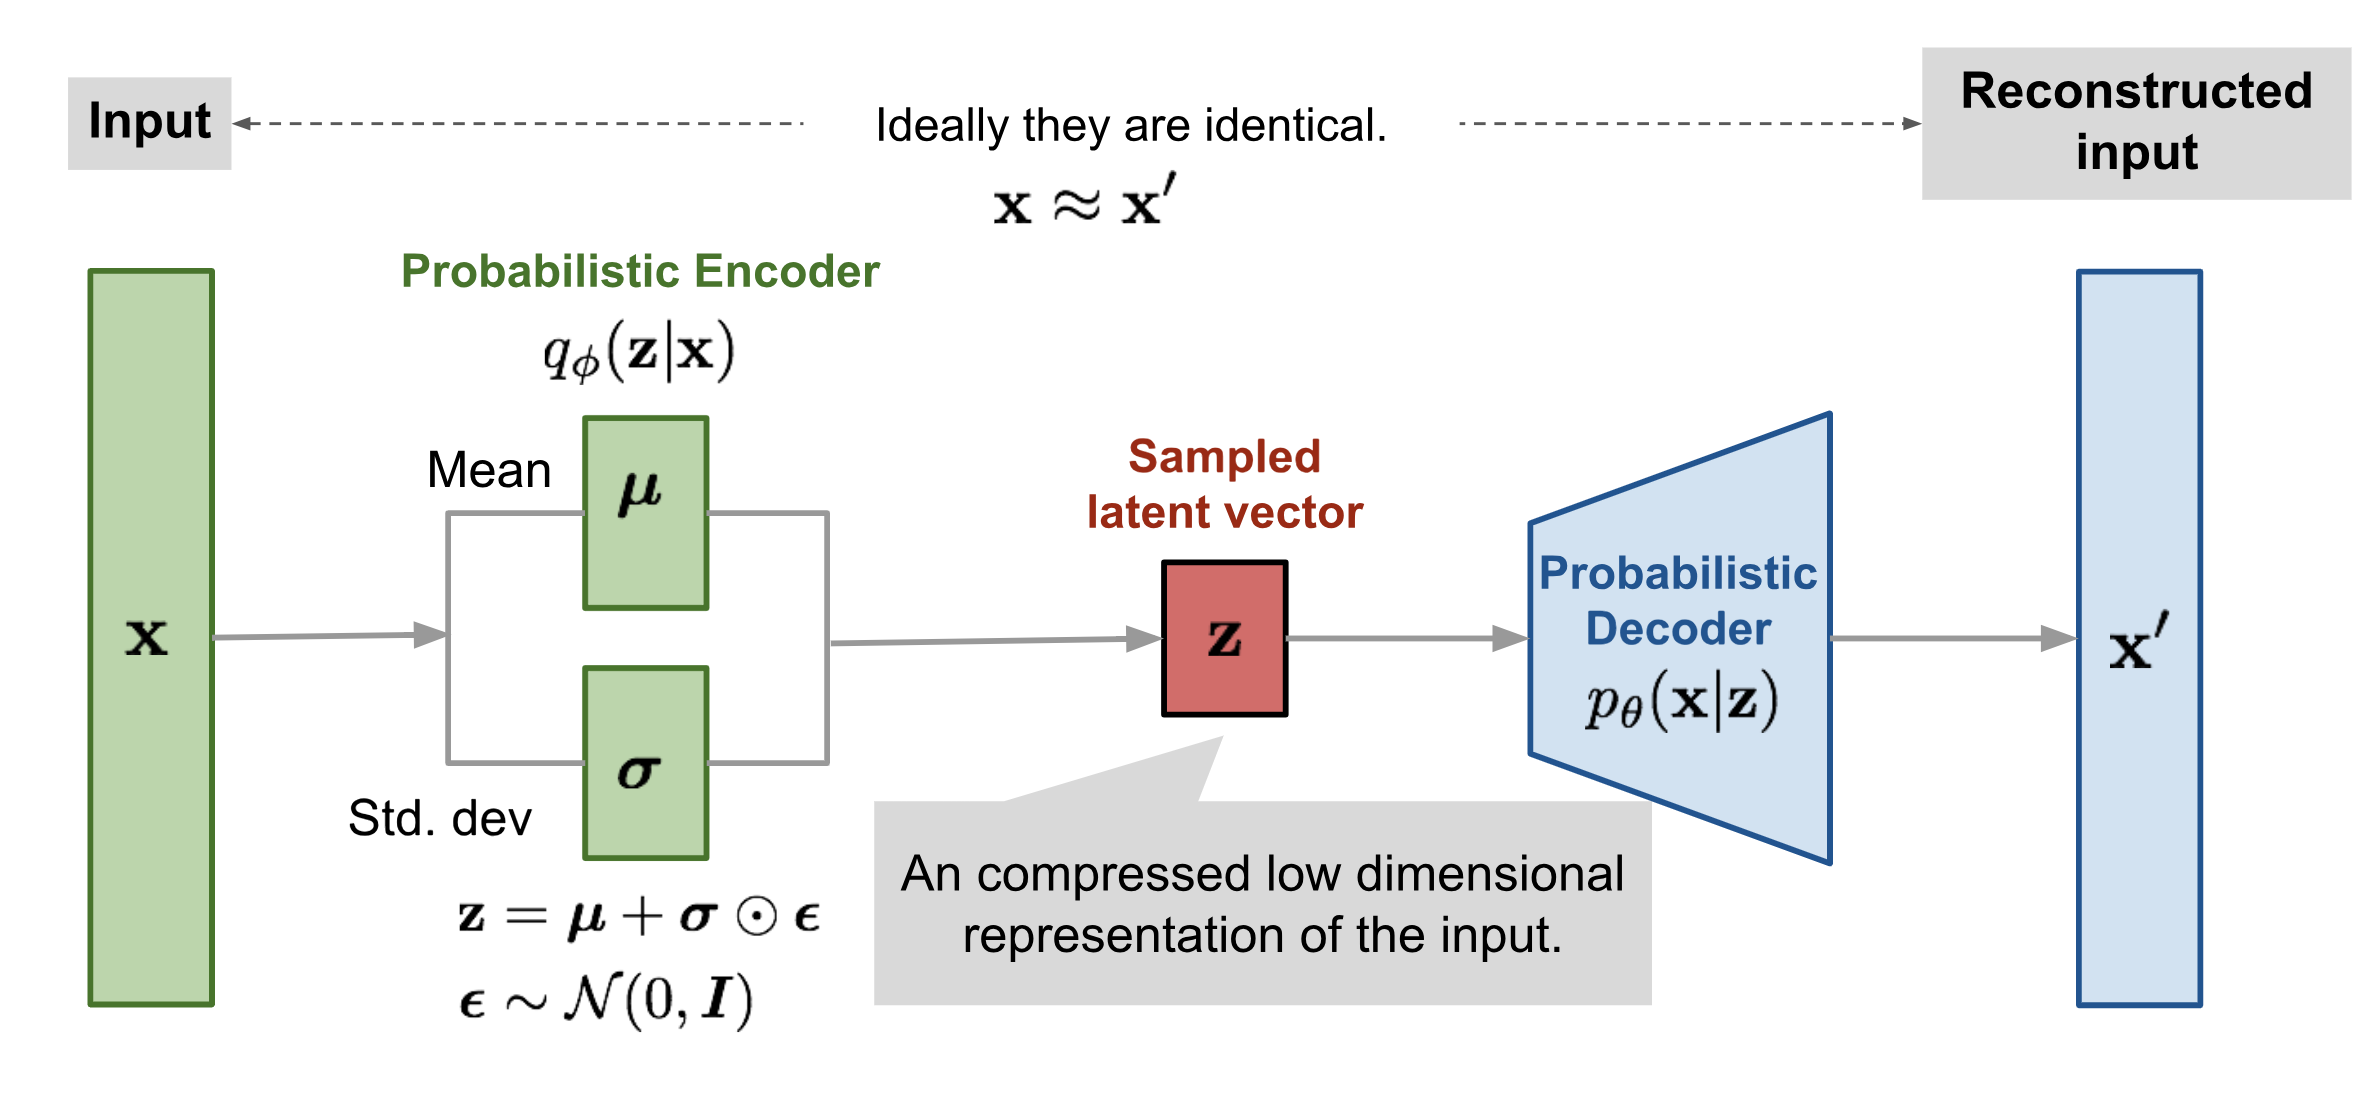
\includegraphics[width=\textwidth]{img/vae-gaussian}
\caption{VAE model with the multivariate Gaussian assumption. \cite{cit:vae}}
\end{figure}

\end{frame}
%--------- END Frame 12 -------------
\begin{frame}{Vector Quantised VAE = VQ-VAE}

\begin{figure}[h]
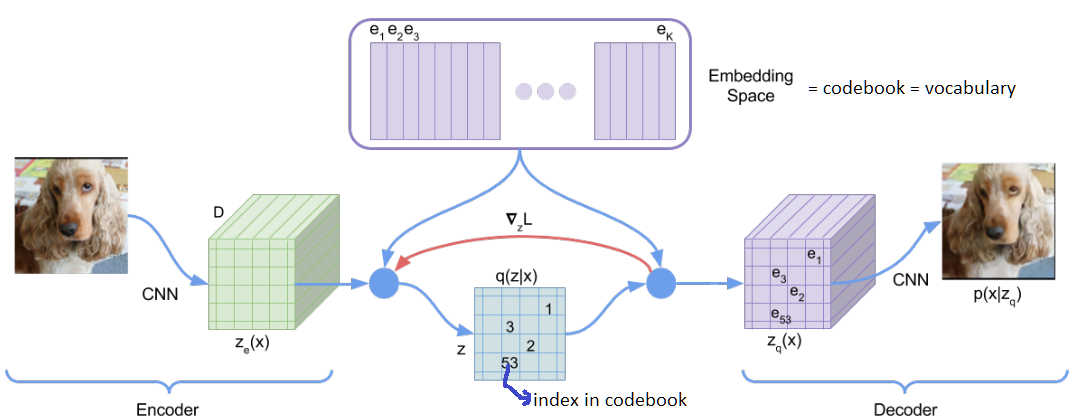
\includegraphics[width=\textwidth]{img/arch}
\caption{The output of the encoder $z(x)$ is mapped to the nearest point $e_i$ in codebook. The gradient $\nabla_zL$ (in red) will push the encoder to change its output, which could alter the configuration in the next forward pass.}
\end{figure}

\end{frame}
%--------- END Frame 12 -------------
\begin{frame}{VQ-VAE Training}
Discrete representation = 1024 of 8096 codebook (vocabulary) embeddings for each image.
\vfill
\textbf{Forward pass:}
\begin{itemize}
\item Split image into a grid of 32x32 = 1024 squares
\item encoder predicts real-valued vector $z_e(x)$ = $E(x)$ for each square
\item $E(x)$ is replaced by an \textbf{index} of nearest neighbor from codebook
\item index = integer = discrete
\item this (32x32x1) map of indices is passed to decoder
\item decoder uses the same codebook to translate indices to vectors and reconstructs the image
\end{itemize}

\end{frame}
%--------- END Frame 12 -------------
\begin{frame}{VQ-VAE Training}

\begin{figure}[h]
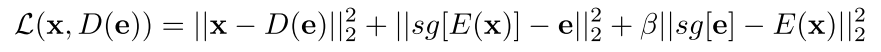
\includegraphics[width=\textwidth]{img/loss}
\caption{Loss = reconstruction + codebook + commitment losses.}
\end{figure}

\textbf{Backwards pass:}
\begin{itemize}
\item reconstruction loss = classic L2 loss
\item codebook loss = pushes codebook vectors closer to encoder output
\item commitment loss = pushes encoder output closer to the nearest codebook vector
\item sg = stop gradient = gradient does not flow into that element
\item nearest neighbor op is not differentiable = copy gradients from decoder input to encoder output = red arrow
\end{itemize}

\end{frame}
%--------- END Frame 12 -------------
\begin{frame}{VQ-VAE Reconstruction examples}

\begin{figure}[h]
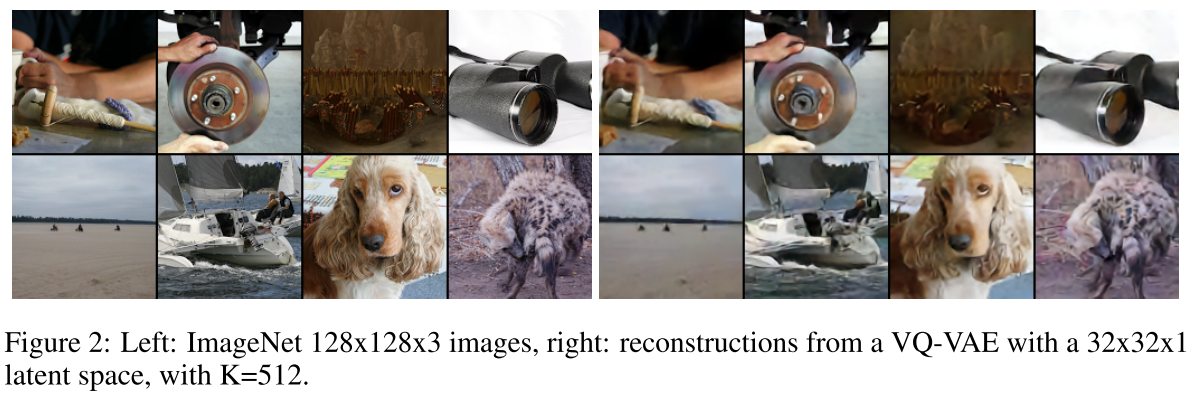
\includegraphics[width=\textwidth]{img/reconstruction}
\end{figure}


\begin{itemize}
\item only slightly blurry images = very good reconstruction
\end{itemize}

\end{frame}
%--------- END Frame 12 -------------
\begin{frame}{VQ-VAE Generation of images}

\begin{itemize}
\item after training the VQ-VAE
\item train a per-pixel auto-regressive generative model on the discrete 32x32x1 space of the trained VQ-VAE
\item then sample from this auto-regressive model conditioned on a class label
\item sample = 32x32x1 
\item input the sample into decoder $\implies$ generated image
\end{itemize}

\vfill
\textbf{Why train this extra model?}\\
Latent variables sampled from the learned prior at test time are close to what the decoder network has observed during training which results in more coherent outputs.


\end{frame}
%--------- END Frame 12 -------------
\begin{frame}{VQ-VAE Generation examples}

\begin{figure}[h]
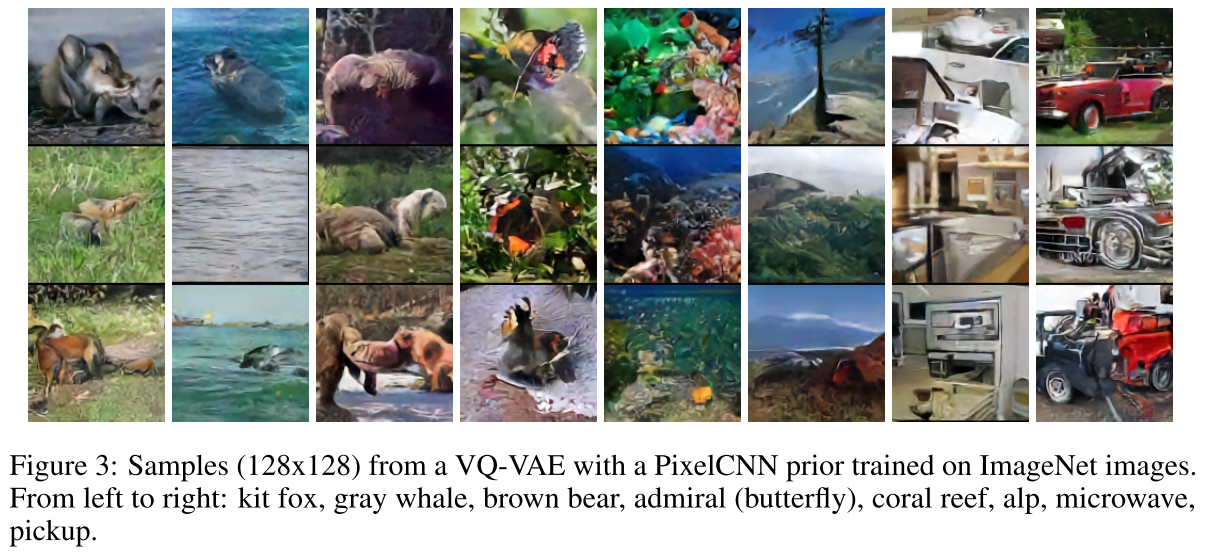
\includegraphics[width=\textwidth]{img/generated}
\end{figure}

Auto-regressive models:
\begin{itemize}
\item PixelCNN = used in this paper
\item PixelSNAIL \cite{snail} = used in VQ-VAE-2 = hierarchical version
\end{itemize}

\end{frame}
%--------- END Frame 12 -------------

%--------- END Frame 12 -------------
\begin{frame}{Sources}
\begin{thebibliography}{0}

  \bibitem[1]{cit:paper} 1.Oord, Aaron van den, Oriol Vinyals, and Koray Kavukcuoglu. "Neural discrete representation learning." arXiv preprint arXiv:1711.00937 (2017). \url{https://arxiv.org/abs/1711.00937} 
  
  \bibitem[2]{cit:vae} 2. VAE overview blog post. \url{https://lilianweng.github.io/lil-log/2018/08/12/from-autoencoder-to-beta-vae.html}
  
  \bibitem[3]{snail} 3. Chen, Xi, et al. "Pixelsnail: An improved autoregressive generative model." International Conference on Machine Learning. PMLR, 2018. \url{https://arxiv.org/abs/1712.09763}
  
  \bibitem[4]{dp} 4. Razavi, Ali, Aaron van den Oord, and Oriol Vinyals. "Generating diverse high-fidelity images with vq-vae-2." arXiv preprint arXiv:1906.00446 (2019). \url{https://arxiv.org/abs/1906.00446}
  
  \bibitem[5]{dp} 5. VQ-VAE implementation \url{https://github.com/nadavbh12/VQ-VAE/tree/master/vq_vae}
  
\end{thebibliography}

\end{frame}

 
\end{document}
